\chapter{Einleitung}
\section{Motivation}
Im zunehmenden Maße finden sich mobile Endgeräte (z.B. Tablet) als Marketing-,\newline Informations- und Imageelement, aber auch als Teil von Prozessen im Retail- als auch im Industrieumfeld wieder. Diese ersetzen oder erweitern bestehende Lösungen (z.B. Kiosk, Digital-Signage, Laptops, Industrie PCs) um interaktive Elemente und unterstützen so Unternehmen in ihren Geschäftsprozessen. 
Bei der eingesetzten Lösung ist es aus Sicht des Retail und Industriekunden wichtig, die Handhabung und das Erlebnis des Gerätes für den Anwender zu erhalten. Die Einsatzgebiete reichen dabei von Tablets in Produktionsprozessen zu Zwecken der Qualitätssicherung (eigene Applikationen mit Dokumentationsfunktionen) bis hin zu Multimedia-Terminals im stationären Handel. Um diese verschiedenen Szenarien realisieren zu können, ist es notwendig eine stabile, sichere und wartbare Plattform zu konstruieren, die zum einen die Anwendung in unterschiedlichen Einsatzgebieten ermöglicht und zum anderen für den Betriebsführer leicht bereitzustellen und zu warten ist.
\paragraph*{}
Um den hier angeführten allgemeinen Anforderungen ihrer Kunden gerecht zu werden, benötigt Kapsch die passendste Softwarelösung im Bereich Security für die hierfür in Betracht gezogenen Tablets. Um diese Softwarelösung zu ermitteln, wurde ein Projektteam des fünften Jahrgangs der HTBLVA Spengergasse, Fachbereich Informatik, mit der Aufgabe der Eroierung dieser Lösung und  der Erstellung eines Konzepts betraut. Das Projekt KTI – Kapsch Tablet Infrastructure wird von dem Projektmanager Philip Steinhäuser geleitet  und besteht aus den Teammitgliedern Sebastian Götze, Samuel Hammer,\newline Michael Kaufmann und Konstanze Müller. Das Projektteam steht in engem Kontakt mit dem Project owner, welcher durch die Mitarbeiter Bernhard Bruckner und Jürgen Krammer vertreten ist. 
\paragraph*{}
Kapsch unterstützt das Projekt mit diversen Hilfeleistungen sowie Technischer Supports, intellektueller Hilfe und finanzieller Unterstützung beim Kauf des Tablets, welches nach Beendigung des Projekts wieder in den Besitz von Kapsch übergehen wird.

\newpage

\section{Projektpartner}
\begin{figure}[H]

\includegraphics[scale=1.0]{Images/kapsch_logo}
\caption{Kapsch Logo}
\end{figure}
Die Kapsch Group setzt sich aus 3 Hauptunternehmen zusammen:
\begin{itemize}
	\item Kapsch TrafficCom
	\item Kapsch CarrierCom
	\item Kapsch BusinessCom
\end{itemize}

\paragraph*{}
Die Kapsch TrafficCom ist internationaler Anbieter von Technologien, Lösungen und Dienstleistungen für den Intelligent Transportation Systems (ITS) Markt. 
\paragraph*{}
Die Kapsch CarrierCom ist globaler Lösungspartner für Telco-Carrier und Communication-Provider sowie Railway-Operator. 
\paragraph*{} 
Unser konkreter Projektpartner ist die Kapsch BusinessCom.
Mit 1.400 Mitarbeitern, einem Umsatz von knapp 300 Millionen Euro und Niederlassungen in Österreich, Tschechien, Slowakei, Ungarn, Rumänien und Polen positioniert sich das Unternehmen als einer der führenden ICT-Servicepartner in Zentral- und Osteuropa. Kapsch setzt auf Partnerschaften mit führenden Branchengrößen wie Apple, Cisco, Google, HP oder Microsoft, um seinen rund 17.000 Kunden den bestmöglichen Service gewährleisten zu können.

\newpage

\section{Ursprungsproblem}
Die Aufgabe von Kapsch an das Projektteam ist es, verschiedene Softwarelösungen zum Systemschutz von Android-Tablets zu testen. Die vom Project owner zum Test gewünschten Softwarelösungen sind.
\begin{itemize}
	\item MDM
	\item MDM + Container
	\item Samsung Knox
\end{itemize}
Zusätzlich besteht noch die Möglichkeit einer \textbf {Linux Manipulation}, welche jedoch für Kapsch aus rechtlichen Gründen nicht in Frage kommt, da diverse Garantieverletzungen auftreten und zusätzlich enorme Kosten aufgrund von hohen Entwicklungskosten und langen Entwicklungszeiten, bis das System einwandfrei funktioniert, anfallen würden.
\paragraph*{}
Zu diesen Schutzsystemmöglichkeiten soll ein Untersuchungsbericht angefertigt werden. In diesem werden die Ergebnisse  festgehalten und verglichen, um das beste System für die Kunden von Kapsch zu ermitteln.
\paragraph*{}
Auf Basis dieses Untersuchungsberichts soll dann die passendste Softwarelösung ausgewählt werden, welche in ein Konzept eingebaut wird. Ein Teil dieses Konzepts beinhaltet die Implementierung der ausgewählten Softwarelösung auf ein Tablet, welches dann als Prototyp deklariert wird. 
\paragraph*{}
Der Untersuchungsbericht in Kombination mit dem Prototyp ist das Ergebnis, welches über den Ausgang dieses Projekts entscheidet.


\section{Vorgehensweise}
\subsection{Vorbereitung}
\begin{itemize}
	\item Vorbereitungsmeeting mit Kapsch
	\item Einlesen in Technologie
	\item Erste Recherchen
\end{itemize}
\subsection{Planung}
\begin{itemize}
	\item Projektantrag
	\item Vorstudie
	\item PSP (Projektstrukturplan)
	\item OSP (Objektstrukturplan)
	\item Timetable bzw. Gantt-Chart
	\item Lastenheft
	\item Pflichtenheft
	\item Projekthandbuch
	\item Checklist Template
	\item Research Template
	\item Untersuchungsbericht
	\item Diplomarbeit
\end{itemize}
\subsection{Durchführung}
\begin{itemize}
	\item Recherche
	\item Erstellung des Untersuchungsberichtes
	\item Auswahl der passenden Lösung
	\item Konzept erstellen
	\item Ausgewählte Lösung in Konzept einarbeiten
	\item Konzept teilweise umsetzen - Konfiguration der Lösung auf Tablet (Prototyp)
\end{itemize}
\subsection{Ergebnis}
\begin{enumerate}
	\item Untersuchungsbericht
	\item Prototyp
\end{enumerate}

\subsection{Organigramm}
\begin{figure}[H]
	\centering
	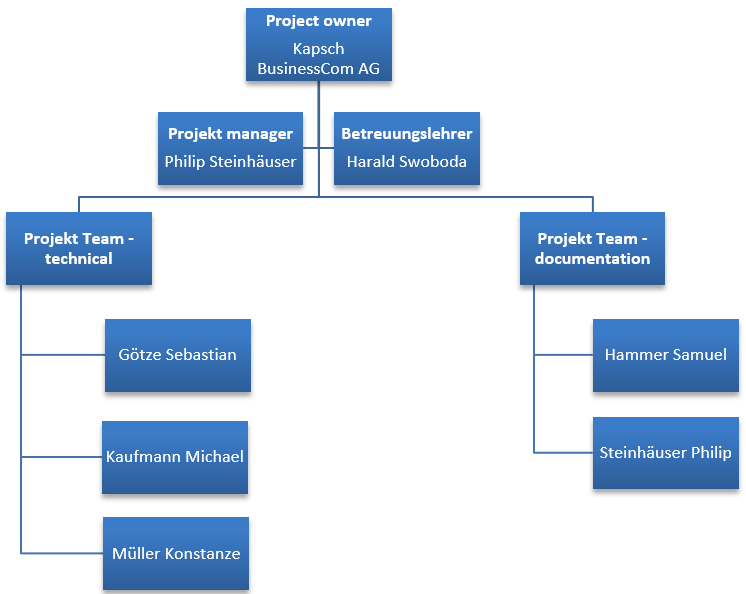
\includegraphics[scale=0.6]{Images/organigramm}
	\caption{Projekt-Organigramm}
\end{figure}
Die Aufgaben des Projekts wurden so verteilt, dass das Dokumentationsteam sämtliche Projektmanagementaufgaben und das Technikteam alle Research- und Testungsaufgaben übernimmt.
\begin{figure}[H]
	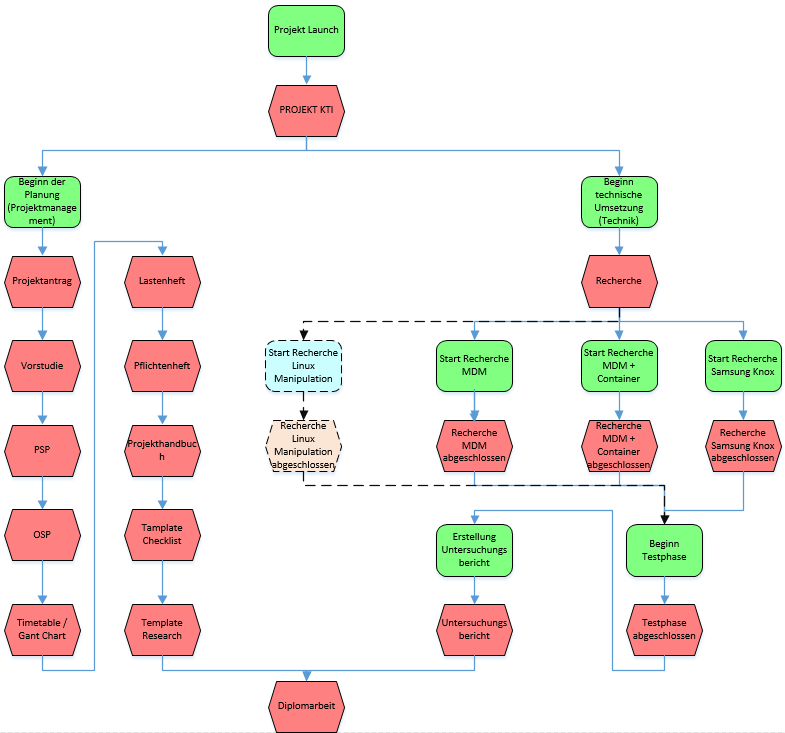
\includegraphics[scale=0.7]{Images/arbeitsteilung}
	\caption{Aufgabenverteilung - Diagramm}
\end{figure}
Dieses Ablaufdiagramm zeigt auf der einen Seite die Reihenfolge der erstellten Dokumente, so wie beispielsweise, dass der OSP und der Timetable/Gantt Chart auf dem PSP aufbaut, da dieser zuvor erstellt wurde und diese drei Dokumente konsistent sein müssen.
\paragraph*{}
Auf der Technik Seite wiederum sieht man, dass zuerst eine umfangreiche Recherche nötig ist bzw. war, bevor die Wahl der passendsten Softwarelösung getroffen werden kann/konnte, welche dann schlussendlich für das Konzept und in weiterer Folge für die Konfiguration des Prototyps verwendet werden konnte/wurde.


\newpage

Wenn man sich unsere Vorgehensweise nun Schritt für Schritt auf die beiden Sub Teams aufgeteilt anschauen würde, würde folgendes Bild entstehen:

\begin{table}[H]
	\begin{tabular}{| c | p{6.5cm} | p{7.5cm} |}
		\hline
		\textbf \# & \textbf{Dokumentation} & \textbf{Technik}
		\\\hline %----------new line----------
		1 
		&%-----
		\begin{itemize}
			\item Erstellung des Projektantrages
			\item Erstellung der Vorstudie
			\item Erstellung PSP
			\item Erstellung OSP
		\end{itemize}
		&%-----
		-
		\\\hline %----------new line----------
		2
		&%-----
		\begin{itemize}
			\item Erstellung des Gantt-Chart
			\item Erstellung Lastenheft
			\item Erstellung Pflichtenheft
		\end{itemize}
		&%-----
		\begin{itemize}
			\item Beginn der Recherchephase
			\begin{itemize}
				\item Recherche Linux Manipulation
				\item Recherche MDM
				\item Recherche MDM+Container
				\item Recherche Samsung Knox
			\end{itemize}
		\end{itemize}
		\\\hline %----------new line----------
		3
		&%-----
		\begin{itemize}
			\item Erstellung Projekthandbuch
			\item Erstellung Research Template
			\item Erstellung Checklist Template
		\end{itemize}
		&%-----
		\begin{itemize}
			\item Festhalten der Rechercheergebnisse in Templates
			\item Recherchephase abgeschlossen
			\begin{itemize}
				\item Recherche Linux Manipulation abgeschlossen
				\item Recherche MDM abgeschlossen
				\item Recherche MDM+Container abgeschlossen
				\item Recherche Samsung Knox abgeschlossen
			\end{itemize}
		\end{itemize}
		\\\hline %----------new line----------
		4
		&%-----
		\begin{itemize}
			\item Erstellung Diplomarbeit
		\end{itemize}
		&%-----
		\begin{itemize}
			\item Beginn der Testphase
			\item Erstellung des Untersuchungsberichts
		\end{itemize}
		\\\hline %----------new line----------
		5
		&%-----
		\begin{itemize}
			\item Fertigstellung Diplomarbeit
			\item Fertigstellung Projekthandbuch
		\end{itemize}
		&%-----
		\begin{itemize}
			\item Abschluss der Testphase
			\item Fertigstellung des Untersuchungsberichts
		\end{itemize}
		\\\hline %----------new line----------
	\end{tabular}
	\caption{Projektablauf}
\end{table}

\newpage

\section{Arbeitsaufteilung}
In unserem Projekt wurde die Arbeit so aufgeteilt, dass kein Teammitglied zu viel oder zu wenig, sondern genau richtig ausgelastet ist, um die Freude und Motivation an der Arbeit über die Dauer der Projektarbeit immer konstant hoch zu halten. Hier zu sehen ist, was welches Projektmitglied an welchem Dokument gearbeitet hat oder welche Softwarelösung von ihm recherchiert und textuell beschrieben wurde.

\subsection{Sebastian Götze}
Sebastian war Verantwortlicher für die Recherche an den Softwarelösungen Mobile Device Management sowie Linux Manipulation, welches jedoch lediglich aus Informationszwecken, und nicht aufgrund seiner Verwendung recherchiert wurde. Weiters arbeitete er an Dokumenten wie dem Projektantrag, der Vorstudie, dem Pflichtenheft sowie dem Projekthandbuch mit. Von ihm stammen außerdem das Checklist Template sowie das Research Template, welche für die Recherche sowie das Testing der einzelnen Softwarelösungen verwendet wurden.
%	\begin{itemize}
%		\item Projektantrag
%		\item Vorstudie
%		\begin{itemize}
%			\item status quo
%			\item MDM
%		\end{itemize}
%		\item Template Checklist
%		\item Template Research
%		\item Pflichtenheft
%		\begin{itemize}
%			\item Unternehmensperspektive
%			\item Funktionale Beschreibung
%		\end{itemize}
%		\item Projekthandbuch
%		\begin{itemize}
%			\item Project Assignment
%			\item Plan of objects of consideration
%			\item Project Work-Package Specification
%			\item Project Rules
%		\end{itemize}
%		\item Gantt-Chart
%		\item Mobile Device Management (MDM)
%		\begin{itemize}
%			\item Recherche
%			\item Testing
%			\item Untersuchungsbericht
%			\item Diplomarbeit
%		\end{itemize}
%		\item Linux Manipulation
%		\begin{itemize}
%			\item Recherche
%			\item Untersuchungsbericht
%			\item Diplomarbeit
%		\end{itemize}
%		\item Prototyp
%	\end{itemize}


\subsection{Samuel Hammer}
Samuel war Verantwortlicher für das Erstellen sämtlicher Präsentationen sowie für die Schriftführung bei unseren Projectownermeetings, welche im Anschluss an diese von ihm in Form von Besprechungsprotokollen dokumentiert und festgehalten wurden. Weiters arbeitete er am Projektantrag, der Vorstudie, dem Projekthandbuch, dem Pflichtenheft sowie der Diplomarbeit mit. Von ihm stammt außerdem die erste Version unserer Zeitplanung in Form eines Gantt Charts, welche bzw. welches als Grundlage für die folgenden Versionen und als Unterstützung der Planung von etwaigen Terminen von Abgaben, sowie zur Projektfortschrittskontrolle verwendet wurde.
%	\begin{itemize}
%		\item Projektantrag
%		\item Vorstudie
%		\begin{itemize}
%			\item Critical Appraisal
%			\item Android Technology Analysis
%		\end{itemize}
%		\item Projekthandbuch
%		\begin{itemize}
%			\item Project Assignment
%			\item Description of Pre- and Post-Project Phase
%			\item Project Work-Package Specification
%			\item Project Bar Chart
%			\item Minutes - Project Co-Ordination
%		\end{itemize}
%		\item Pflichtenheft
%		\begin{itemize}
%			\item Funktionen
%			\item Betriebsbedingungen
%			\item Härtung der mobilen Endgeräte
%		\end{itemize}
%		\item Besprechungsprotokolle
%		\item Präsentationen
%		\begin{itemize}
%			\item Statuspräsentationen
%			\begin{itemize}
%				\item 09.12.2014
%				\item 08.01.2015
%				\item 19.02.2015
%				\item 19.03.2015
%				\item 16.04.2015
%			\end{itemize}
%			\item Abschlusspräsentation Englisch
%			\item Abschlusspräsentation Deutsch
%		\end{itemize}
%		\item Gantt-Chart
%		\item Diplomarbeit
%	\end{itemize}

\subsection{Michael Kaufmann}
Michael war Verantwortlicher für die Recherche an der Softwarelösung Samsung Knox, sowie deren Implementierung nach Beendigung der Research- und Testingphase. Weiters arbeitete er am Projektantrag, der Vorstudie, dem Projekthandbuch sowie dem Pflichtenheft mit. Zudem sind von ihm Gantt-Chart Versionen, welche eine große Rolle in der Planung und dem reibungslosen Ablauf unseres Projekts spielten, erstellt worden.
%	\begin{itemize}
%		\item Projektantrag
%		\item Vorstudie
%		\begin{itemize}
%			\item Samsung Knox
%		\end{itemize}
%		\item Projekthandbuch
%		\begin{itemize}
%			\item Project assignment
%			\item Project Objectives
%			\item Project Work-Package Specification
%		\end{itemize}
%		\item Pflichtenheft
%		\begin{itemize}
%			\item System Architecture
%			\begin{itemize}
%				\item Hardware
%				\item Software
%			\end{itemize}
%		\end{itemize}
%		\item Gantt-Chart
%		\item Samsung Knox
%		\begin{itemize}
%			\item Recherche
%			\item Testing
%			\item Untersuchungsbericht
%			\item Diplomarbeit
%			\item Implementierung
%		\end{itemize}
%		\item Prototyp
%	\end{itemize}

\subsection{Konstanze Müller}
Konstanze war Verantwortliche für die Recherche der Softwarelösung Mobile Device Management mit Container, bei welcher sie einige für den später erstellten Untersuchungsbericht relevante Daten sammeln und textuell in den jeweiligen Checklist und Research Templates festhalten konnte. Weiters arbeitete sie an dem Projektantrag, der Vorstudie, dem Projekthandbuch sowie dem Pflichtenheft mit. Gemeinsam mit Philip erstellte sie alle zwei Wochen einen Statusbericht.
%	\begin{itemize}
%		\item Projektantrag
%		\item Vorstudie
%		\begin{itemize}
%			\item MDM + Container
%		\end{itemize}
%		\item Projekthandbuch
%		\begin{itemize}
%			\item Project Assignment
%			\item Project environment Graphic
%			\item Project Environment Table
%			\item Project Work-Package Specification
%			\item Project Risk Analysis
%			\item Project Status Reports
%		\end{itemize}
%		\item Pflichtenheft
%		\begin{itemize}
%			\item Target Groups
%			\item Quality Criteria
%		\end{itemize}
%		\item Besprechungsprotokolle
%		\item Statusberichte
%		\item Mobile Device Management (MDM) + Container
%		\begin{itemize}
%			\item Recherche
%			\item Testing
%			\item Untersuchungsbericht
%			\item Diplomarbeit
%		\end{itemize}
%		\item Prototyp
%	\end{itemize}

\newpage

\subsection{Philip Steinhäuser (Projektleiter)}
Philip war neben seiner Tätigkeit als Projektleiter auch Verantwortlicher für das Projekthandbuch, die Meilensteintrendanalyse, die Statusberichte, das Abnahmeprotokoll sowie für das Project Controlling und Zeitmanagement des Projekts.  Er arbeitete am Projektantrag, der Vorstudie, dem Objektstrukturplan (OSP), dem Projektstrukturplan (PSP), dem Pflichtenheft, dem Projekthandbuch sowie der Diplomarbeit mit. Von ihm wurde weiters die eben schon erwähnte Meilensteintrendanalyse sowie das Abnahmeprotokoll verfasst. Weiters zählte die regelmäßige Aktualisierung des Projekthandbuchs sowie die Vertretung des Projektteams gegenüber dem Projektpartner und den Lehrern zu seinen Aufgaben. 
%\begin{itemize}
%	\item Projektantrag
%	\item Vorstudie
%	\begin{itemize}
%		\item Management Summary
%		\item Task
%		\item SWOT - Analyse
%	\end{itemize}
%	\item Gantt-Chart
%	\begin{itemize}
%		\item laufende Aktualisierung und Projektfortschrittskontrolle
%	\end{itemize}
%	\item Kooperationsvereinbarung
%	\item Meilensteinplan
%	\item Meilensteintrendanalyse
%	\item Objektstrukturplan - OSP
%	\item Projektstrukturplan - PSP
%	\item Pflichtenheft
%	\begin{itemize}
%		\item Requirement Specification
%		\item Embedding in Organisation
%		\item Milestones
%	\end{itemize}
%	\item Projekthandbuch
%	\begin{itemize}
%		\item Project Assignment
%		\item Project Organisation Chart
%		\item Project Organisation
%		\item Work Breakdown Structure (WBS)
%		\item Project Work-Package Specification
%		\item Milestoneplan
%		\item Project Communication
%		\item Project Responsibility Matrix
%		\item Project Documentation
%		\item Project Co-Ordination
%		\item Project Status Report
%		\item Laufende Aktualisierung und Ausarbeitung des einzelnen Punkte des Projekthandbuchs
%	\end{itemize}
%	\item Statusberichte
%	\item Abnahmeprotokoll (Acceptance Testing Protocol - ATP)
%	\item Diplomarbeit
%\end{itemize}